\section{Tổng quan về Trò chơi Bloxorz và Môi trường Mô phỏng}
\label{sec:game_overview}

Để xây dựng các tác tử giải thuật có khả năng suy luận và giải quyết
bài toán Bloxorz, bước tiên quyết là hình thức hóa luật chơi vật lý
dưới góc nhìn của ngành Trí tuệ Nhân tạo. Chương này trình bày chi tiết
khung phân loại môi trường PEAS, mô hình động học không gian của khối,
các quy tắc tương tác địa hình phức tạp, và kiến trúc phần mềm phân tầng
được thiết kế cho hệ thống mô phỏng.

\subsection{Hình thức hóa Môi trường Tác tử theo Khung PEAS}
\label{subsec:peas_framework}
Theo lý thuyết của Russell và Norvig \cite{russell2020aima}, bài toán
Bloxorz được đặc tả đầy đủ qua bộ tiêu chí PEAS được tổng hợp tại
Bảng \ref{tab:peas_spec}.

\begin{table}[H]
\centering
\caption{Đặc tả môi trường tác tử Bloxorz theo khung PEAS}
\label{tab:peas_spec}
\small
\begin{tabularx}{\textwidth}{l X}
\toprule
\textbf{Thành phần} & \textbf{Mô tả chi tiết trong Đồ án} \\
\midrule
\textbf{Hiệu năng} &
- Tối thiểu hóa số bước lật khối đưa khối về đích.\\
& - Tối ưu hóa tổng chi phí tích lũy đường đi.\\
& - Tránh hoàn toàn việc rơi vào ô rỗng hoặc làm sập gạch cam.\\
& - Tối thiểu hóa thời gian tính toán và lượng bộ nhớ RAM tiêu thụ.\\
\midrule
\textbf{Môi trường} &
- Mặt bằng lưới tọa độ $2\text{D}$ rời rạc $\mathbb{Z}^2$
kích thước $W \times H$.\\
& - Các loại ô sàn: Gạch bền, Gạch mong manh, Ô thoát, Ô rỗng.\\
& - Hệ thống công tắc: Công tắc tròn, Công tắc chữ X, Cổng phân thân.\\
& - Các nhóm cầu nối đóng/mở động theo trạng thái boolean.\\
\midrule
\textbf{Bộ tác động} &
- Khối nguyên vẹn: Các hành động lật khối 4 hướng:
$\{\text{UP}, \text{DOWN}, \text{LEFT}, \text{RIGHT}\}$.\\
& - Khối phân thân: Lăn khối lập phương đơn hoặc chuyển đổi
quyền điều khiển giữa hai khối (\texttt{SWITCH\_CUBE}).\\
\midrule
\textbf{Bộ cảm biến} &
- Nhận thức hoàn hảo tọa độ và tư thế định hướng của khối.\\
& - Nhận thức toàn bộ trạng thái cấu hình của bàn cờ (vị trí đích,
trạng thái đóng/mở của tất cả các cầu nối).\\
\bottomrule
\end{tabularx}
\end{table}

Dựa trên các đặc tính vận hành, môi trường Bloxorz được phân loại
chính xác vào các nhóm đặc trưng sau:
\begin{itemize}[--]
    \item \textbf{Quan sát toàn phần:}
    Tại bất kỳ thời điểm nào, tác tử đều nắm bắt đầy đủ thông tin về
    trạng thái hình học của khối và trạng thái logic của toàn bộ bàn cờ.
    Không có thông tin ẩn hay yếu tố sương mù chiến tranh.

    \item \textbf{Tất định:}
    Khi tác tử thực hiện một hành động di chuyển $a \in A$ từ trạng thái $s$,
    trạng thái kế tiếp $s'$ hoàn toàn được xác định chắc chắn $100\%$ theo
    các phương trình động học vật lý, không có nhiễu ngẫu nhiên.

    \item \textbf{Tuần tự:}
    Mỗi quyết định di chuyển tại thời điểm hiện tại ảnh hưởng trực tiếp
    đến các cấu hình khả dĩ trong tương lai (ví dụ: tư thế khi tiếp cận
    công tắc hoặc cầu nối).

    \item \textbf{Tĩnh:}
    Môi trường bàn cờ hoàn toàn đứng yên trong lúc tác tử suy nghĩ giải
    thuật; trạng thái cầu và ô sàn chỉ thay đổi khi có hành động kích hoạt
    từ chính khối của tác tử.

    \item \textbf{Rời rạc:}
    Cả không gian (tọa độ lưới nguyên) và thời gian (các bước lật theo
    lượt) đều có tính chất rời rạc.

    \item \textbf{Đơn tác tử:}
    Trong môi trường chỉ có một tác tử duy nhất giải quyết bài toán,
    không có sự cạnh tranh hay phối hợp đối kháng từ các tác tử khác.
\end{itemize}

Hình \ref{fig:gui_3d} minh họa giao diện đồ họa 3D trực quan của hệ thống
mô phỏng Bloxorz trên nền tảng màn chơi khởi đầu (Stage 01).

\begin{figure}[H]
    \centering
    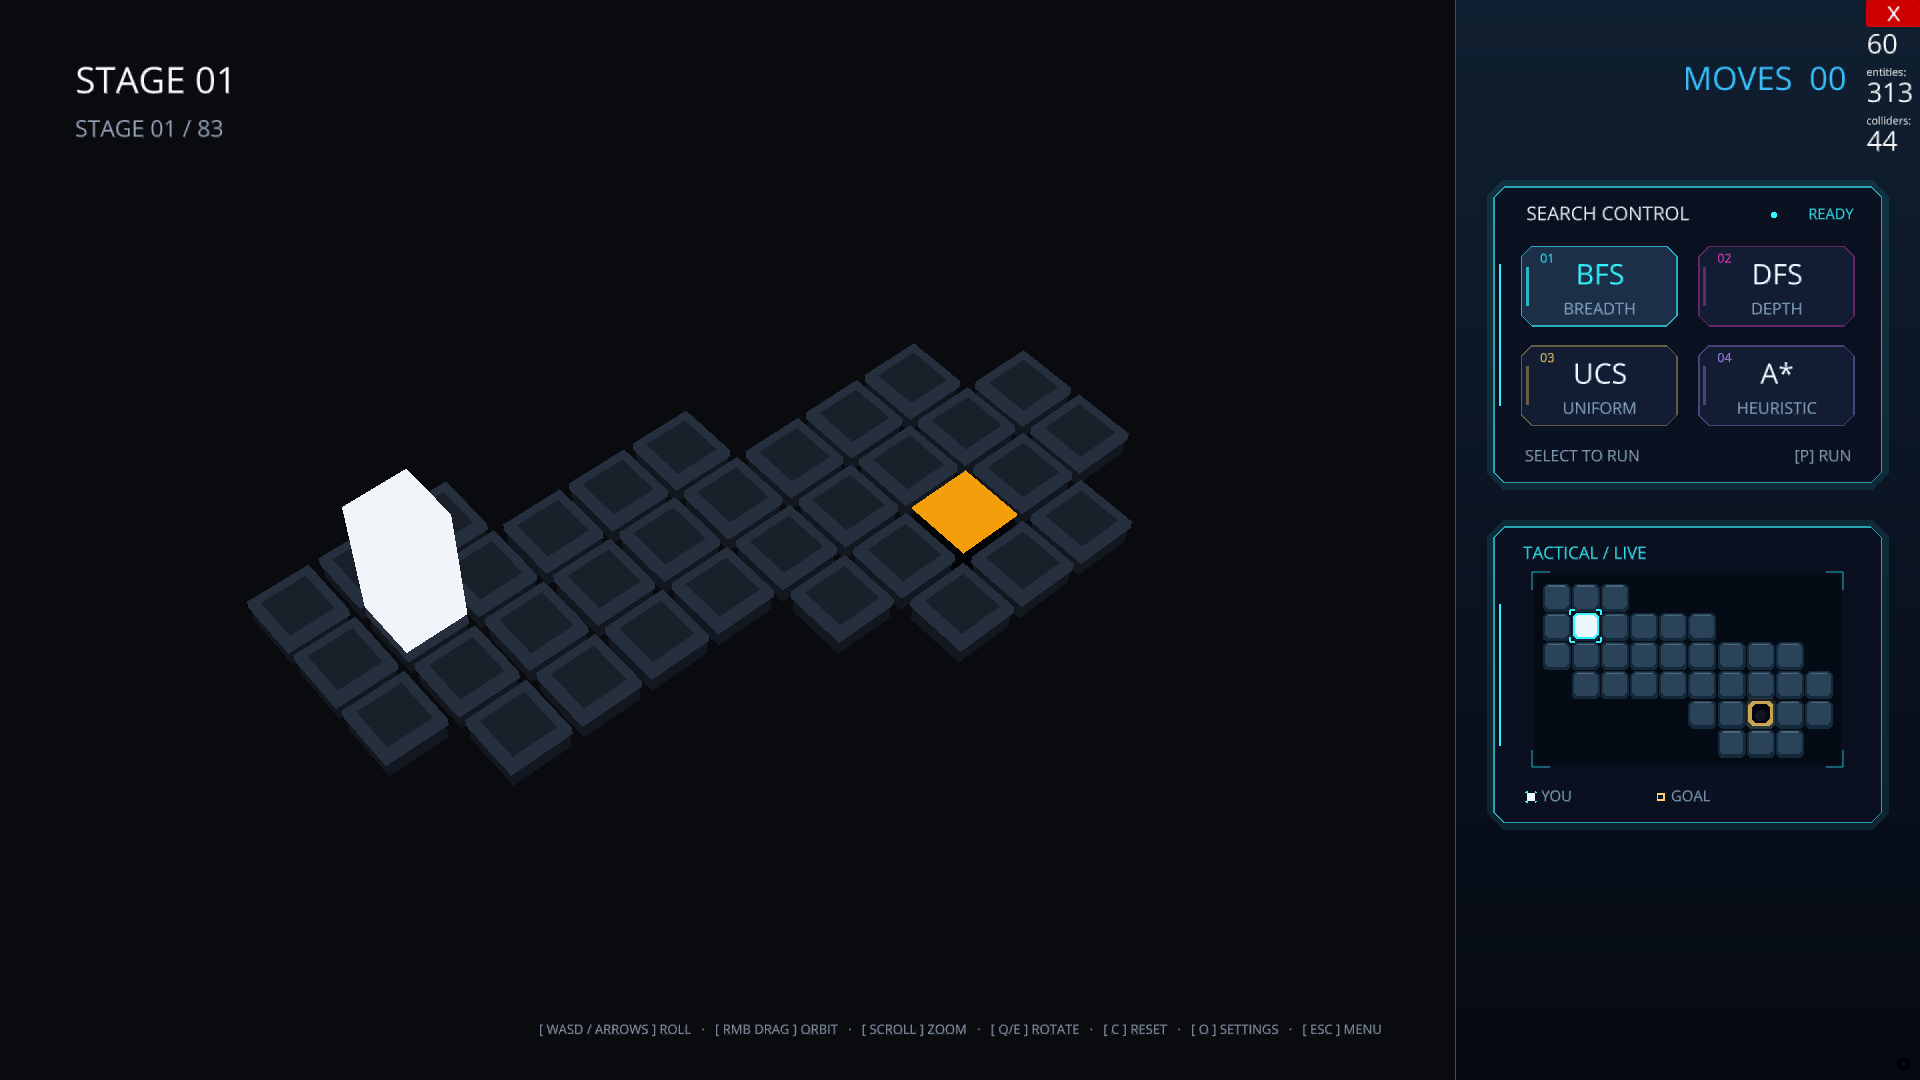
\includegraphics[width=0.88\textwidth]{images/game_gui_3d.png}
    \caption{Giao diện 3D trực quan với Tactical Minimap
    và bảng điều khiển giải thuật}
    \label{fig:gui_3d}
\end{figure}

Giao diện quan sát trong Hình \ref{fig:gui_3d} thể hiện đầy đủ các thành
phần cảm biến và tương tác của môi trường tác tử. Khối hộp chữ nhật
kích thước $1 \times 1 \times 2$ được đặt tại ô xuất phát với tư thế đứng
chuẩn mực. Ô đích màu xanh lục neon phát sáng thể hiện vị trí mục tiêu
cần tiếp cận. Bảng hiển thị ở góc trên cung cấp thông tin màn chơi hiện tại
và số bước lật đã thực hiện. Bản đồ thu nhỏ Tactical Minimap tại góc dưới
bên phải chiếu toàn cảnh mặt bằng lưới hai chiều $\mathbb{Z}^2$, phản ánh
trực tiếp nguyên lý quan sát toàn phần khi tác tử có thể nhận biết tức thời
vị trí của bản thân và toàn bộ bố cục địa hình xung quanh. Ngoài ra, bảng
điều khiển giải thuật Neon HUD tại góc trên bên phải cho phép người dùng
chọn nhanh một trong bốn giải thuật (BFS, DFS, UCS, A*) để khởi động quá
trình tìm kiếm và tự động hóa điều khiển.

\subsection{Mô hình Động học Khối Không gian}
\label{subsec:kinematics}
Khối Bloxorz nguyên bản là một khối hộp chữ nhật đồng chất kích thước
$1 \times 1 \times 2$. Trạng thái hình học của khối được mô hình hóa
bằng bộ $3$ tham số:
\begin{equation}
    S_{\text{block}} = \langle x, y, \mathcal{O} \rangle
\end{equation}
Trong đó $(x, y) \in \mathbb{Z}^2$ là tọa độ ô gốc (góc trái trên của
phần tiếp xúc sàn), và $\mathcal{O}$ là tư thế định hướng không gian
thuộc tập hợp:
\begin{equation}
    \mathcal{O} \in \{\text{STANDING}, \text{LYING\_X}, \text{LYING\_Y}\}
\end{equation}

Tập hợp các ô lưới bị che phủ bởi khối được xác định tường minh:
\begin{equation}
    \text{Cells}(x, y, \mathcal{O}) =
    \begin{cases}
        \{(x, y)\} & \text{khi } \mathcal{O} = \text{STANDING} \\
        \{(x, y), (x+1, y)\} & \text{khi } \mathcal{O} = \text{LYING\_X} \\
        \{(x, y), (x, y+1)\} & \text{khi } \mathcal{O} = \text{LYING\_Y}
    \end{cases}
\end{equation}

Khi thực hiện phép lật theo một trong 4 hướng chính
$a \in \{\text{RIGHT}, \text{LEFT}, \text{UP}, \text{DOWN}\}$,
hàm chuyển tiếp trạng thái $T(S_{\text{block}}, a)$ biến đổi tọa độ và tư thế
theo Bảng quy tắc chuyển động \ref{tab:kinematics_rules}.

\begin{table}[H]
\centering
\caption{Bảng chuyển tiếp động học trạng thái khối Bloxorz}
\label{tab:kinematics_rules}
\small
\begin{tabular}{lll}
\toprule
\textbf{Tư thế $\mathcal{O}$}
& \textbf{Hướng $a$}
& \textbf{Trạng thái mới $\langle x', y', \mathcal{O}' \rangle$} \\
\midrule
\multirow{4}{*}{\textbf{STANDING}}
& RIGHT & $\langle x+1, y, \text{LYING\_X} \rangle$ \\
& LEFT  & $\langle x-2, y, \text{LYING\_X} \rangle$ \\
& UP    & $\langle x, y-2, \text{LYING\_Y} \rangle$ \\
& DOWN  & $\langle x, y+1, \text{LYING\_Y} \rangle$ \\
\midrule
\multirow{4}{*}{\textbf{LYING\_X}}
& RIGHT & $\langle x+2, y, \text{STANDING} \rangle$ \\
& LEFT  & $\langle x-1, y, \text{STANDING} \rangle$ \\
& UP    & $\langle x, y-1, \text{LYING\_X} \rangle$ \\
& DOWN  & $\langle x, y+1, \text{LYING\_X} \rangle$ \\
\midrule
\multirow{4}{*}{\textbf{LYING\_Y}}
& RIGHT & $\langle x+1, y, \text{LYING\_Y} \rangle$ \\
& LEFT  & $\langle x-1, y, \text{LYING\_Y} \rangle$ \\
& UP    & $\langle x, y-1, \text{STANDING} \rangle$ \\
& DOWN  & $\langle x, y+2, \text{STANDING} \rangle$ \\
\bottomrule
\end{tabular}
\end{table}

\noindent
\textbf{Trạng thái Phân thân:}
Tại các màn chơi nâng cao, khi khối bước vào ô phân thân (\texttt{TELEPORT}),
khối $1 \times 1 \times 2$ bị tách rời thành hai khối lập phương
$1 \times 1 \times 1$ độc lập: $B_1 = (x_1, y_1)$ và $B_2 = (x_2, y_2)$.
Lúc này, tác tử điều khiển một khối tích cực (xác định bởi chỉ số
$i_{\text{active}} \in \{0, 1\}$). Hành động của tác tử mở rộng thêm
lệnh hoán đổi:
\begin{equation}
    a = \texttt{SWITCH\_CUBE}
    \implies i_{\text{active}}' = 1 - i_{\text{active}}
\end{equation}
Mỗi khối lập phương di chuyển từng ô một theo các hướng
$\{ \text{UP}, \text{DOWN}, \text{LEFT}, \text{RIGHT} \}$.

\noindent
\textbf{Điều kiện Hợp nhất:}
Hai khối lập phương $B_1$ và $B_2$ tự động tái hợp nhất thành khối
$1 \times 1 \times 2$ nguyên bản khi và chỉ khi chúng nằm ở hai ô kề
cạnh nhau trên lưới:
\begin{equation}
    \text{Merge}(B_1, B_2) \iff
    (|x_1 - x_2| = 1 \land y_1 = y_2)
    \lor (|y_1 - y_2| = 1 \land x_1 = x_2)
\end{equation}
Nếu kề theo trục hoành ($x$), khối mới có tư thế $\text{LYING\_X}$; nếu kề
theo trục tung ($y$), khối mới có tư thế $\text{LYING\_Y}$.

Hình \ref{fig:gameplay_split} trực quan hóa cơ chế phân thân khối đặc biệt
trên màn chơi nâng cao (Stage 08).

\begin{figure}[H]
    \centering
    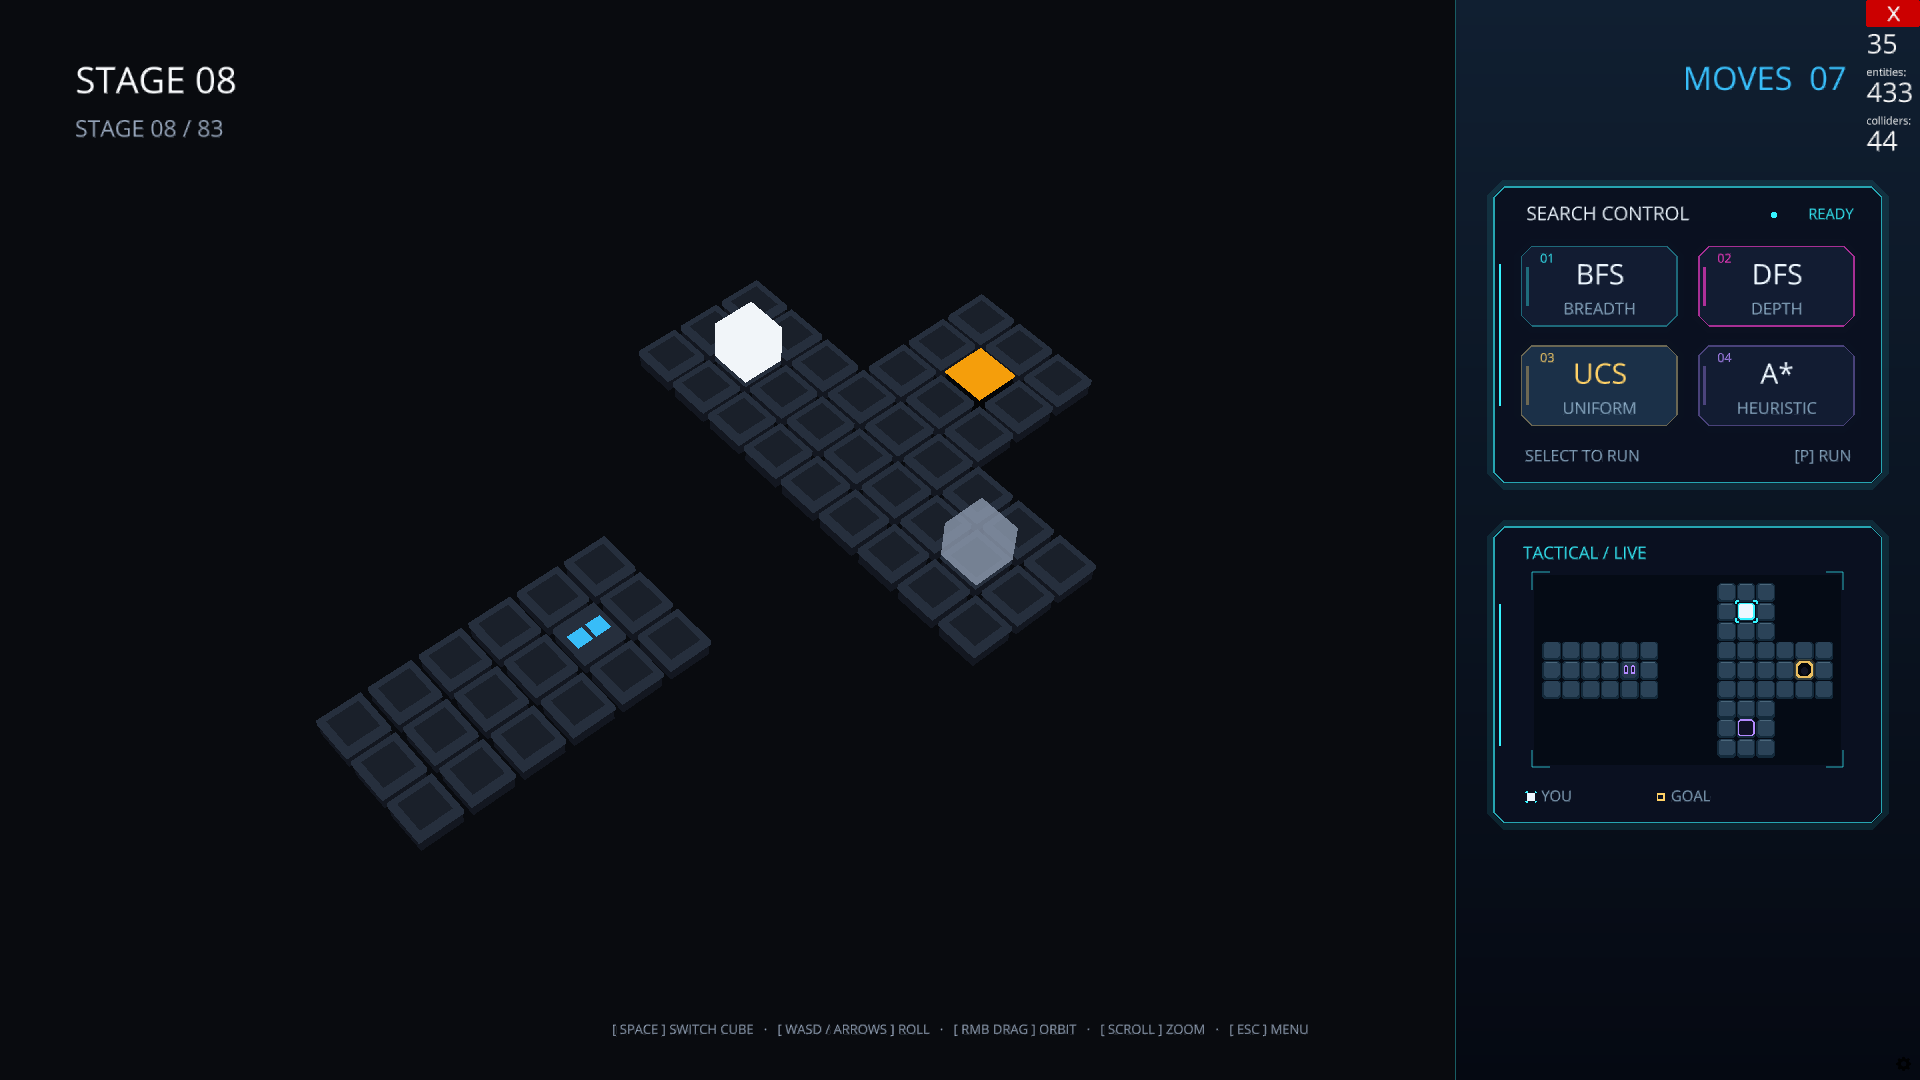
\includegraphics[width=0.88\textwidth]{images/gameplay_split.png}
    \caption{Cơ chế phân tách thành hai khối lập phương
    độc lập qua ô dịch chuyển}
    \label{fig:gameplay_split}
\end{figure}

Như quan sát trong Hình \ref{fig:gameplay_split}, sau khi kích hoạt ô
dịch chuyển, khối chính bị chia thành hai khối lập phương đơn lẻ nằm ở
hai phân vùng bản đồ độc lập. Khối đang nhận quyền điều khiển tích cực
được làm nổi bật với màu sắc viền sáng, trong khi khối thụ động mang sắc
thái dịu hơn nhằm giúp người quan sát phân biệt rõ ràng. Tactical Minimap
đồng thời cập nhật hai điểm định vị phân tách, cho phép theo dõi tương tác
song song của cả hai thực thể trước khi điều hướng chúng hội tụ về các ô
liền kề để tái tạo lại khối hộp chữ nhật nguyên vẹn.

\subsection{Cơ chế Địa hình Nâng cao và Tương tác Môi trường}
\label{subsec:terrain_mechanics}
Không gian Bloxorz bao gồm các ô gạch có đặc tính tương tác vật lý khác nhau:

\begin{enumerate}[1.]
    \item \textbf{Gạch bền và Ô rỗng:}
    Gạch bền chịu được khối ở mọi tư thế. Ô rỗng là vùng không gian
    ngoài bàn cờ; nếu bất kỳ phần nào của khối lấn vào ô rỗng mà không có
    điểm đỡ, khối sẽ lập tức mất thăng bằng và rơi tự do, dẫn đến trạng
    thái thất bại.

    \item \textbf{Ô mục tiêu:}
    Mục tiêu tối thượng của màn chơi là đưa khối về ô đích $(x_g, y_g)$.
    Tuy nhiên, điều kiện chiến thắng đòi hỏi khối bắt buộc phải ở tư thế
    dựng đứng:
    \begin{equation}
        \text{Victory} \iff
        \mathcal{O} = \text{STANDING} \land (x, y) = (x_g, y_g)
    \end{equation}
    Nếu khối nằm ngang đi qua ô đích, nó không rơi vào hố mà chỉ được tính
    như đi qua một ô bình thường.

    \item \textbf{Gạch cam mong manh:}
    Mô phỏng bề mặt có giới hạn chịu lực uốn. Khi khối nằm ngang
    ($\text{LYING\_X}$ hoặc $\text{LYING\_Y}$), trọng lực được phân bố
    đều trên hai ô, gạch cam chịu lực an toàn. Tuy nhiên, nếu khối dựng đứng
    ($\text{STANDING}$) trên ô gạch cam, áp lực tập trung làm sập gạch và
    khối rơi xuyên qua sàn.
\end{enumerate}

Hình \ref{fig:gameplay_fragile} minh họa địa hình gạch cam mong manh
trên màn chơi Stage 04.

\begin{figure}[H]
    \centering
    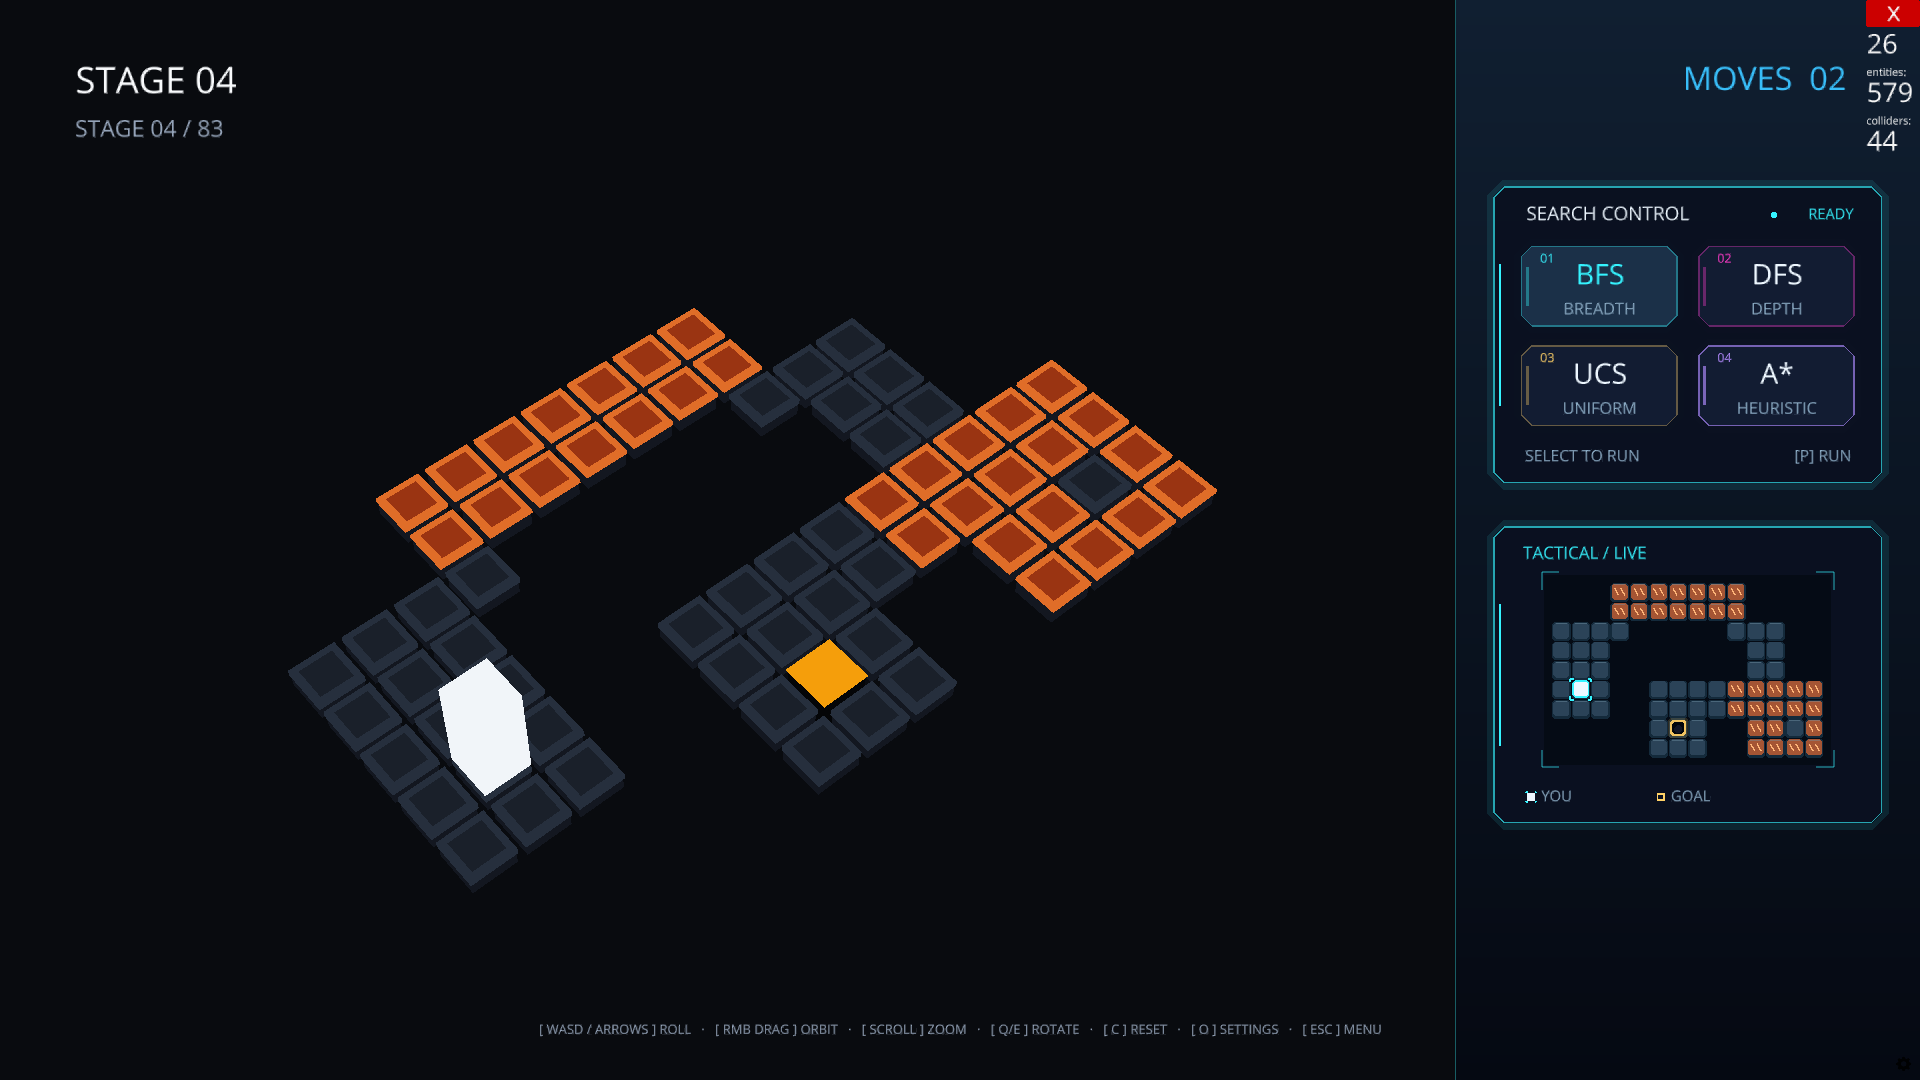
\includegraphics[width=0.88\textwidth]{images/gameplay_fragile.png}
    \caption{Cơ chế chịu lực có điều kiện của dải gạch
    cam mong manh trên Stage 04}
    \label{fig:gameplay_fragile}
\end{figure}

Trong Hình \ref{fig:gameplay_fragile}, dải gạch màu cam kéo dài tạo thành
nhịp cầu nguy hiểm ngăn cách khu vực xuất phát và ô đích. Điểm cốt lõi của
cơ chế này là tính bất đối xứng về khả năng chịu tải: tác tử hoàn toàn có
thể lăn khối nằm ngang qua các ô màu cam này mà không gặp trở ngại; tuy
nhiên, chỉ cần một thao tác dựng khối thẳng đứng trên bất kỳ ô cam nào,
sàn sẽ lập tức nứt vỡ và khiến khối rơi vào trạng thái thất bại. Vì vậy,
trong không gian trạng thái, các trạng thái đứng trên gạch cam bị loại bỏ
như nhánh cụt chết người, hoặc được gán chi phí phạt rất cao trong hàm
đánh giá chi phí của giải thuật UCS.

\begin{enumerate}[resume,leftmargin=*]
    \item \textbf{Công tắc Cơ học và Cầu lật Động:}
    Hệ thống cầu nối có hai trạng thái: đóng (hoạt động như ô rỗng) hoặc
    mở (chịu lực như gạch bền). Trạng thái cầu chịu sự điều khiển của hai
    nhóm công tắc:
    \begin{itemize}[--]
        \item \textit{Công tắc Tròn (Công tắc Mềm):} Kích hoạt bởi bất kỳ
        sự tiếp xúc nào, bất kể khối ở tư thế nằm hay đứng.
        \item \textit{Công tắc Chữ X (Công tắc Nặng):} Đòi hỏi áp lực tập
        trung lớn, chỉ kích hoạt khi khối dựng đứng $\text{STANDING}$ toàn bộ
        trọng lượng lên ô công tắc. Khi khối nằm đè qua công tắc chữ X,
        công tắc hoàn toàn không phản ứng.
    \end{itemize}
    Mỗi công tắc có thể liên kết với một hoặc nhiều nhóm cầu nối với các
    hành vi đảo trạng thái, luôn mở, hoặc luôn đóng.
\end{enumerate}

Hình \ref{fig:gameplay_bridge} thể hiện cấu trúc địa hình liên kết giữa
hệ thống công tắc và các nhịp cầu lật trên Stage 02.

\begin{figure}[H]
    \centering
    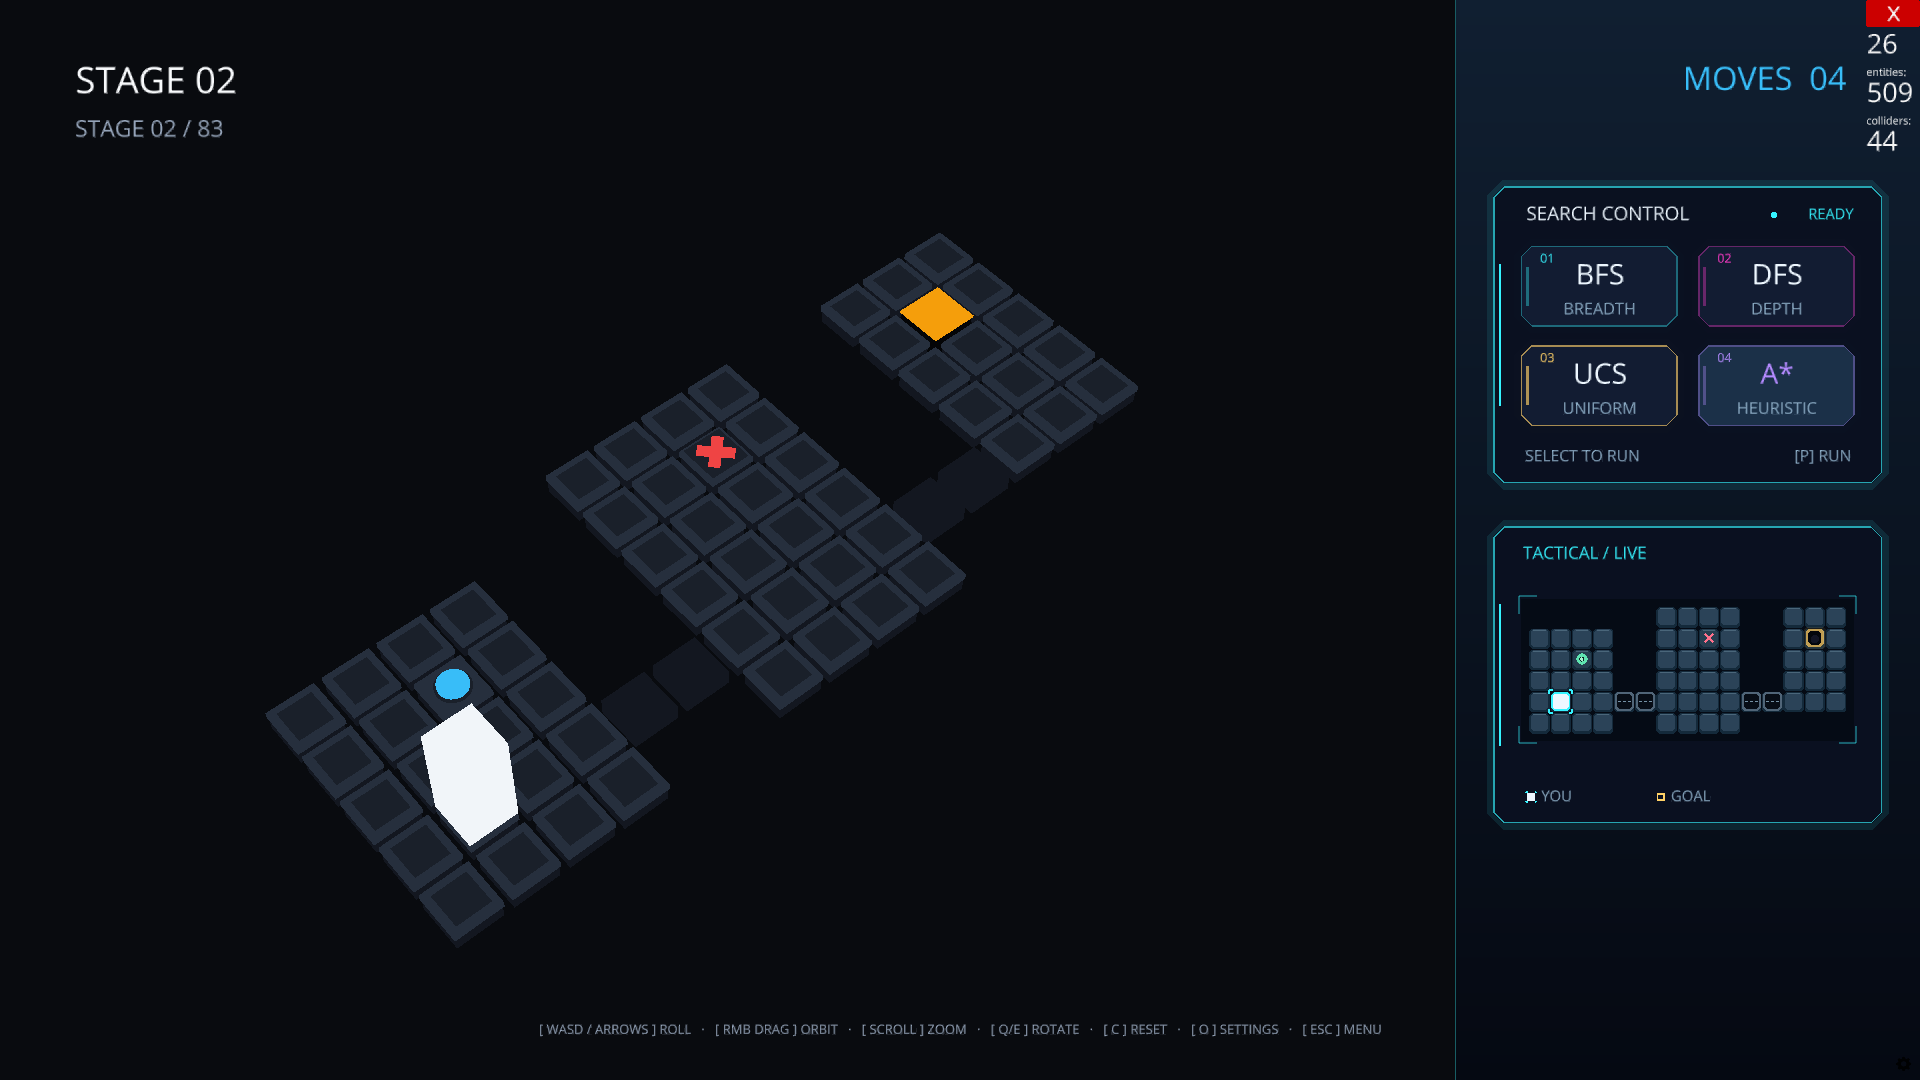
\includegraphics[width=0.88\textwidth]{images/gameplay_bridge.png}
    \caption{Hệ thống công tắc cơ học và các nhịp cầu lật đóng mở trên Stage 02}
    \label{fig:gameplay_bridge}
\end{figure}

Quan sát Hình \ref{fig:gameplay_bridge} cho thấy màn chơi bị chia cắt
thành các hòn đảo độc lập bởi hai khoảng cách vực thẳm. Để tạo đường đi
tới ô đích bên phải, tác tử bắt buộc phải kích hoạt công tắc mềm hình tròn
và công tắc nặng chữ X để nâng các nhịp cầu lên vị trí bằng phẳng. Do
công tắc chữ X chỉ nhận kích hoạt khi khối dựng đứng, tác tử phải tính toán
tọa độ tiếp cận từ trước nhiều bước nhằm đảm bảo tư thế tiếp đất chính xác,
tạo nên tính chất tuần tự chặt chẽ trong quá trình giải quyết bài toán.

\subsection{Kiến trúc Phần mềm Phân tầng}
\label{subsec:architecture}
Để đảm bảo hiệu năng tìm kiếm tính bằng micro-giây trong khi vẫn duy trì
trải nghiệm người dùng 3D mượt mà ở tần số $60\text{ FPS}$, đồ án áp dụng
nguyên lý phân tách mối quan tâm theo kiến trúc phân tầng rõ ràng.

Hệ thống được cấu trúc thành $3$ phân tầng độc lập:
\begin{enumerate}[1.]
    \item \textbf{Tầng Lõi Logic Thuần túy (\texttt{bloxorz.core}):}
    Được viết bằng Python nguyên bản, không phụ thuộc vào bất kỳ thư viện
    đồ họa nào. Bao gồm các cấu trúc dữ liệu biểu diễn trạng thái khối
    nguyên bản, trạng thái khối phân thân và bàn cờ. Tầng này đảm nhận
    nhiệm vụ kiểm tra tính hợp lệ của các bước đi, cập nhật trạng thái cầu,
    và xử lý chuyển đổi trạng thái với tốc độ cao (đạt hơn $50.000$ trạng
    thái mỗi giây).

    \item \textbf{Tầng Thuật toán Trí tuệ Nhân tạo (\texttt{bloxorz.solvers}):}
    Hoạt động hoàn toàn trên tầng lõi, bao gồm lớp cơ sở cho bộ giải,
    cấu trúc nút tìm kiếm và hiện thực của 4 giải thuật BFS, DFS, UCS, A*.
    Tầng này không can thiệp vào giao diện người dùng mà chỉ trả về đối
    tượng kết quả chuẩn hóa bao gồm danh sách hành động, thời gian tìm kiếm,
    số lượng nút mở rộng và bộ nhớ tiêu thụ.
\end{enumerate}

Hình \ref{fig:gameplay_solver} minh họa quá trình tác tử tự động hóa thực
thi chuỗi hành động tìm kiếm trực tiếp trên môi trường đồ họa 3D.

\begin{figure}[H]
    \centering
    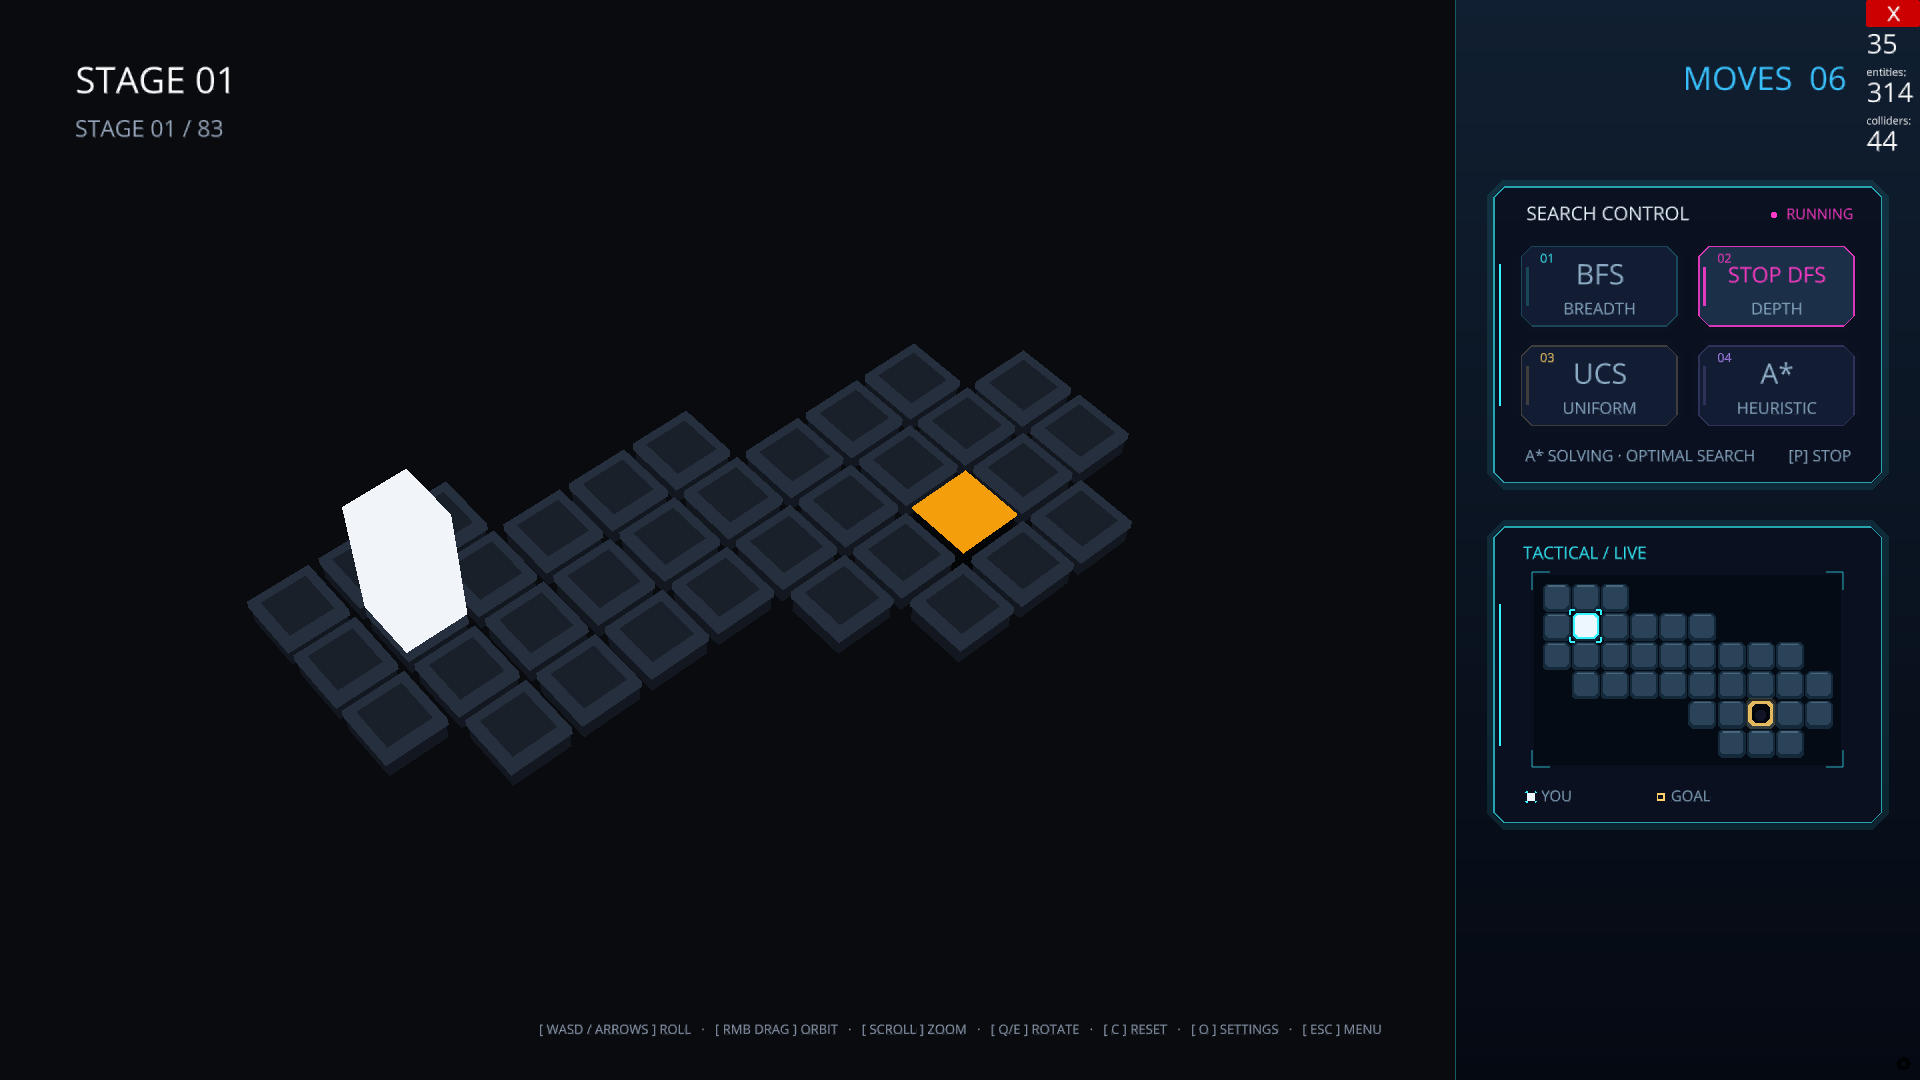
\includegraphics[width=0.88\textwidth]{images/gameplay_solver.png}
    \caption{Tác tử AI thực thi nghiệm tìm kiếm tự động trên giao diện 3D}
    \label{fig:gameplay_solver}
\end{figure}

Khi giải thuật tìm thấy chuỗi bước đi tối ưu, hệ thống kích hoạt chế độ
thực thi tự động như hiển thị trong Hình \ref{fig:gameplay_solver}. Bảng
điều khiển chuyển sang trạng thái hoạt động với tín hiệu phát sáng và dòng
thông báo trạng thái đang chạy. Khối tự động thực hiện các phép lật xoay
tuần tự theo lộ trình tìm được với tốc độ có thể điều chỉnh linh hoạt.
Bộ đếm bước đi trên bảng HUD tăng dần theo từng chuyển động thực tế, giúp
người quan sát dễ dàng theo dõi và kiểm chứng tính đúng đắn của lời giải.

\begin{enumerate}[resume,leftmargin=*]
    \item \textbf{Tầng Giao diện Đồ họa 3D}
    (\texttt{bloxorz.graphics} \& \texttt{bloxorz.ui}):
    Xây dựng trên nền tảng Ursina Engine \cite{amland2020ursina} và Panda3D
    \cite{panda3d2024manual}. Phân tầng này chịu trách nhiệm hiển thị không
    gian ba chiều, tính toán trục xoay linh hoạt để tạo hiệu ứng lật khối
    trơn tru, hiển thị bảng chọn màn chơi và cung cấp bản đồ thu nhỏ trực quan.
\end{enumerate}

Hình \ref{fig:menu_stages} trình bày giao diện lựa chọn màn chơi với hệ thống
phân trang hiện đại của ứng dụng.

\begin{figure}[H]
    \centering
    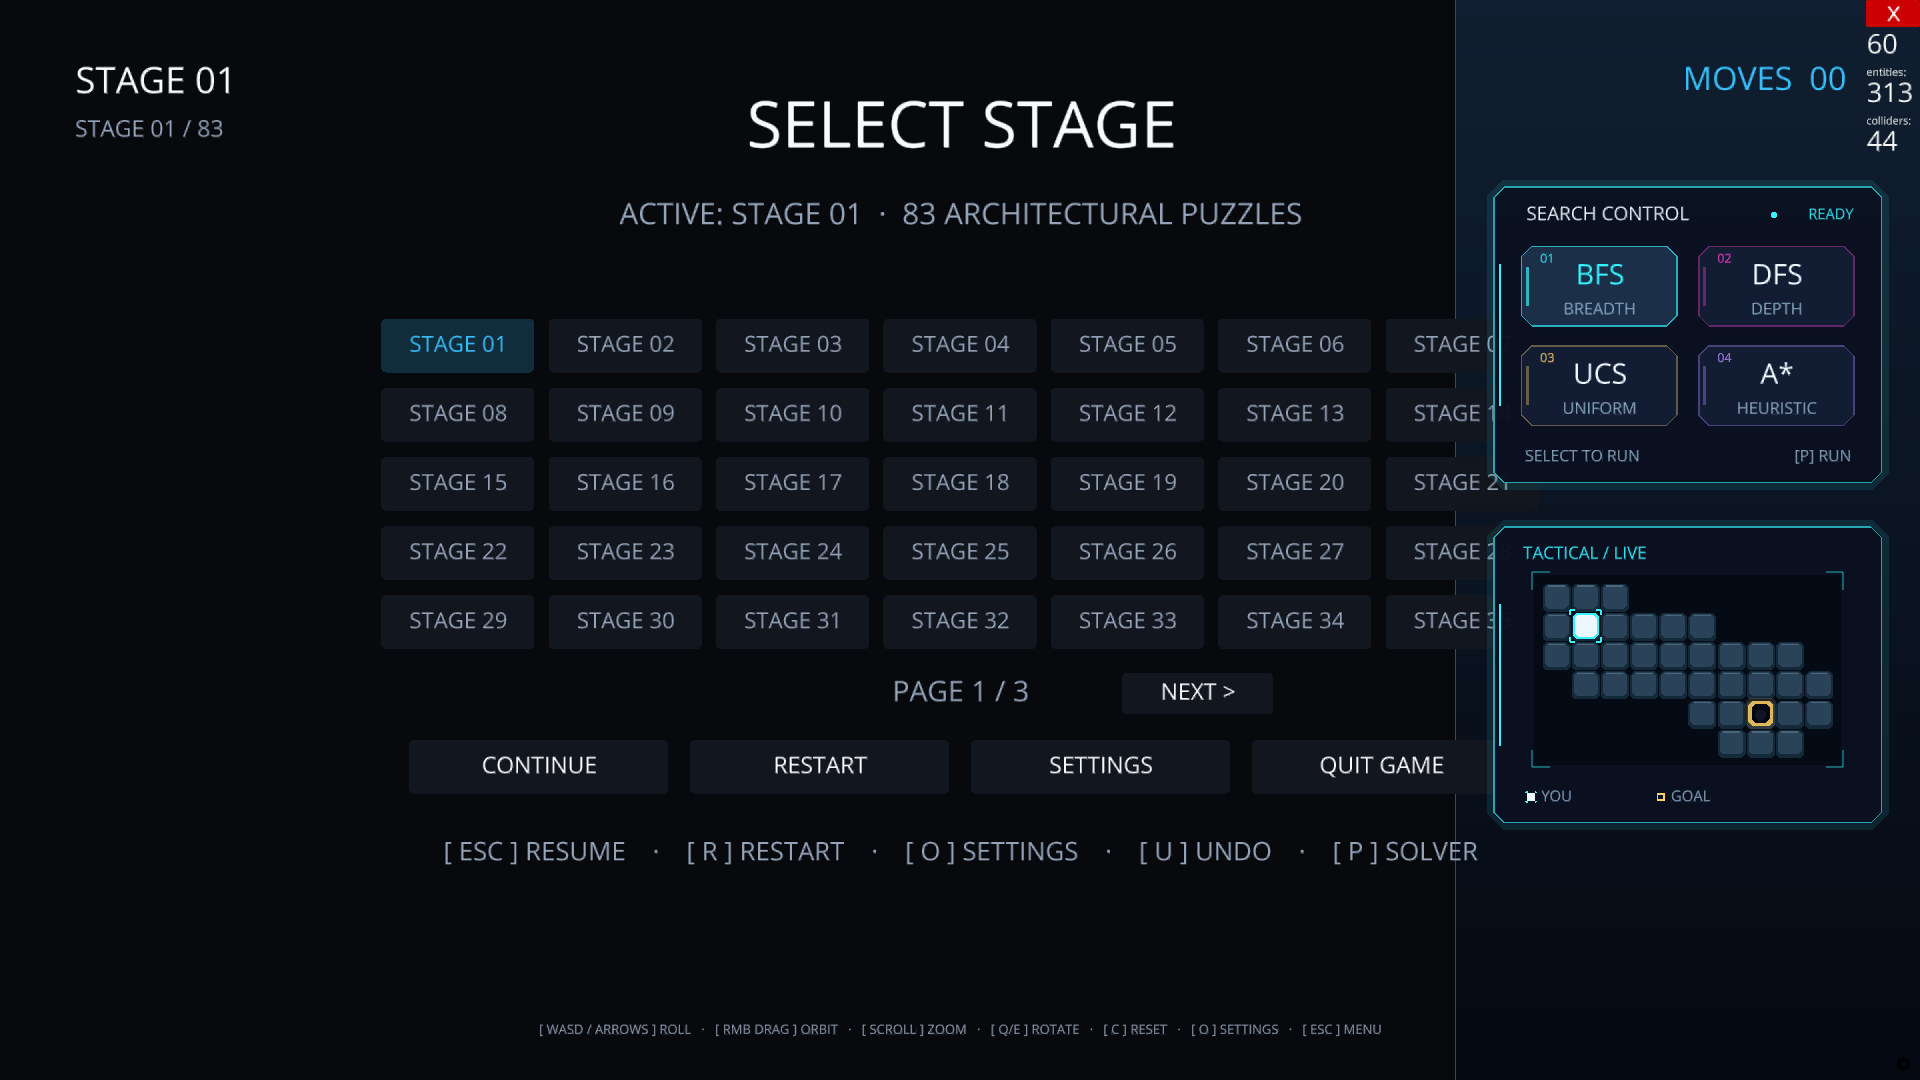
\includegraphics[width=0.88\textwidth]{images/menu_stages.png}
    \caption{Giao diện lựa chọn màn chơi tổ chức theo ma trận phân trang}
    \label{fig:menu_stages}
\end{figure}

Giao diện trong Hình \ref{fig:menu_stages} cho phép người dùng dễ dàng
truy cập và thử nghiệm giải thuật trên bất kỳ màn chơi nào trong toàn bộ
tập dữ liệu gồm 83 màn chơi. Các màn chơi được sắp xếp khoa học theo dạng
lưới 7 cột $\times$ 5 dòng (tương ứng 35 màn chơi trên mỗi trang) kèm theo
các nút chuyển trang trực quan. Màn chơi hiện tại được làm nổi bật để
người dùng tiện theo dõi tiến độ. Phía dưới cùng là thanh công cụ hỗ trợ
các tác vụ nhanh như tiếp tục chơi, chơi lại màn hiện tại, mở cài đặt âm
thanh hoặc quay về màn hình chính.
